\section{Производная функции}
Условие непрерывности функции~$f(x)$ в точке~$a$ можно сформулировать так:
\begin{equation*}
\lim_{\Delta x \to 0} \Delta f = \lim_{\Delta x \to 0} (f(a + \Delta x) - f(a)) = 0
\end{equation*}
где $\Delta x = x - a$ называется \textbf{приращением аргумента}, $\Delta f = f(x) - f(a)$~--- \textbf{приращением функции}.

\index{Функция!одной переменной!дифференцируемая}\index{Производная} Функция~$f(x)$ называется \textbf{дифференцируемой в точке~$a$}, если
$\Delta f \opbr= k \Delta x + o(\Delta x)$ при~$\Delta x \to 0$, где
$\Delta f \opbr= f(x) - f(a)$,
$\Delta x \opbr= x - a$,
$k$~--- константа, называемая \textbf{производной функции~$f(x)$ в точке~$a$} и обозначаемая $f'(a)$.

Из определения следует, что функция, дифференцируемая в точке~$a$, непрерывна в~ней.

Функция называется \textbf{дифференцируемой на} некотором \textbf{множестве}, если она дифференцируема в~каждой точке этого множества.

\index{Функция!гладкая} Точки, в~которых функция дифференцируема, называются \textbf{точками гладкости}.
Функция называется \textbf{гладкой}, если она дифференцируема на всей области определения.

Найдём производную функции~$f(x)$ в точке~$a$.
\begin{equation*}
f'(a) = \lim_{\Delta x \to 0} \frac{\Delta f}{\Delta x} = \lim_{x \to a} \frac{f(x) - f(a)}{x - a}
\end{equation*}

Т.\,о., производная функции~$f(x)$ является функцией~$f'(x)$.

Также можно определить односторонние производные путём рассмотрения соответствующих односторонних пределов.

\textbf{Левой производной функции~$f(x)$ в точке~$a$} называется предел~$\displaystyle \lim_{x \to a-0} \frac{f(x) - f(a)}{x - a}$ и обозначается $f_-'(a)$.

\textbf{Правой производной функции~$f(x)$ в точке~$a$} называется предел~$\displaystyle \lim_{x \to a+0} \frac{f(x) - f(a)}{x - a}$ и обозначается $f_+'(a)$.

\subsection{Геометрический смысл производной}
\begin{wrapfigure}{r}{0pt}
\noindent
\shorthandoff{"}
\begin{tikzpicture}
\drawaxis{-0.5}{4}{-0.5}{3};
\draw (-0.6, 0.5) to[out=80, in=180] (1, 1.35)
	to[out=0, in=-120] (2, 2) coordinate["$c$" {above left}] (c) node {$\bullet$}
	to[out=60, in=135] (4, 1.5)
	node[below left] {$y = f(x)$};
	
\draw[name path=tangent] (c) +(60:1.5) -- +(-120:4);
\coordinate (x) at (\right_x, 0);
\draw[name intersections={of=tangent and x_axis, by=z}]
	pic[draw, "$f'(c)$", angle eccentricity=2.75, angle radius=3mm] {angle = x--z--c};
\end{tikzpicture}
\shorthandon{"}
\end{wrapfigure}

Пусть дана кривая, заданная уравнением~$y = f(x)$, $f(x)$ непрерывна на~$[a; b]$.
Проведём касательную к этой кривой в точке~$c \in (a; b)$.
Заметим, что касательная~--- это прямая, получающаяся в~пределе из хорд, проходящих через точки $(c, f(c))$ и $(c + \Delta x, f(c + \Delta x))$.
Уравнение такой хорды имеет вид
\begin{equation*}
\frac{x - c}{(c + \Delta x) - c} = \frac{y - f(c)}{f(c + \Delta x) - f(c)} \Leftrightarrow
y = f(c) + \frac{f(c + \Delta x) - f(c)}{\Delta x} (x - c)
\end{equation*}

Переходя к пределу при~$\Delta x \to 0$, получим значение углового коэффициента~$k$ касательной:
\begin{equation*}
k = \lim_{\Delta x \to 0} \frac{f(c + \Delta x) - f(c)}{\Delta x} = f'(c)
\end{equation*}

Т.\,о., $y = f(c) + f'(c)(x - c)$~--- уравнение касательной в точке~$c$.

Существование касательной означает, что
\begin{equation*}
\displaystyle \exists \lim_{\Delta x \to 0} \frac{f(c + \Delta x) - f(c)}{\Delta x} = f'(c) \Rightarrow
f(c + \Delta x) - f(c) = f'(c) \Delta x + a\Delta x
\end{equation*}
где $\lim\limits_{\Delta x \to 0} a = 0 \Rightarrow a\Delta x = o(\Delta x)$.
Т.\,о., существование касательной к графику функции~$f(x)$ в точке~$c$ равносильно дифференцируемости функции~$f(x)$ в точке~$c$.

\subsection{Физический смысл производной}
Пусть зависимость пути, пройденного некоторой точкой, от времени выражается функцией~$S(t)$.
Чтобы найти среднюю скорость движения в~промежутке времени $[t_0; t_0 + \Delta t]$, достаточно вычислить $\dfrac{S(t_0 + \Delta t) - S(t_0)}{\Delta t}$.
Перейдём к пределу при~$\Delta t \to 0$, тогда $[t_0; t_0 + \Delta t]$ выродится в~точку, а средняя скорость движения превратится в~мгновенную скорость в точке~$t_0$.
Т.\,о., производная функции~$S(t)$ представляет зависимость мгновенной скорости от времени.

\subsection{Дифференциал функции}
\begin{wrapfigure}{r}{0pt}
\noindent
\begin{tikzpicture}[scale=1.5]
\drawaxis{-2}{2.5}{-0.5}{3};
\draw[name path=curve] (-2, 0.15) to[out=10, in=-135] (0.7, 1.15) coordinate (M)
	to[out=45, in=-100] (1.5, 3)
	node[below left] {$y = f(x)$};
\draw[name path=tangent] (M) +(-135:3) -- +(45:3);
\printcoordsonaxis{M}{x_0}{f(x_0)};

\path[name path=vertical] (1.35, \bottom_y) -- (1.35, \top_y);
% рисуем выступы для указания значения df(x_0)
\draw[dashed,
	name intersections={of=curve and vertical, by=x},
	name intersections={of=tangent and vertical, by=delta_x}]
	(delta_x) +(3mm, 0) -- (delta_x -| 0,0)
	node[left] {$f(x_0) + f'(x_0) \Delta x$}
	(delta_x |- M) +(3mm, 0) -- (M);
% указываем значение df(x_0)
\draw[<->] (delta_x |- M) +(2mm, 0) coordinate (temp_point)
	(delta_x) +(2mm, 0) -- (temp_point)
	node[pos=0.5, right] {$df(x_0)$};

\printcoordsonaxis{x}{x}{f(x)};

% надпись \Delta x
\path (M |- 0,0) -- (x |- 0,0) node[pos=0.5, above] {$\Delta x$};
\end{tikzpicture}
\end{wrapfigure}

\index{d@$d$} \index{Дифференциал} Пусть $f(x)$~--- функция, дифференцируемая в точке~$x_0$, тогда по определению
\begin{equation*}
f(x) - f(x_0) = f'(x_0)(x - x_0) + \alpha
\end{equation*}
где $\alpha = o(x - x_0)$ при~$x \to x_0$.
Слагаемое~$f'(x_0)(x - x_0)$ представляет линейную часть приращения функции.
Его называют \textbf{дифференциалом функции~$f(x)$ в точке~$x_0$} и обозначают $df(x_0) = f'(x_0)\,dx$, где $dx = \Delta x$~--- приращение аргумента.

Можно записать производную, используя дифференциал:
\begin{equation*}
f'(x) = \frac{df}{dx}
\end{equation*}

\subsection{Правила дифференцирования}
Пусть $f(x)$, $g(x)$~--- функции, дифференцируемые в точке~$a$, $C$~--- константа.
\begin{enumerate}
	\item $h(x) = f(x) + g(x)$ дифференцируема в точке~$a$, причём $h'(x) = f'(x) + g'(x)$.
	\begin{proof}
	\begin{equation*}
	h'(a) =
	\lim_{x \to a} \frac{(f(x) + g(x)) - (f(a) + g(a))}{x - a} =
	\lim_{x \to a} \frac{f(x) - f(a)}{x - a} + \lim_{x \to a} \frac{g(x) - g(a)}{x - a} =
	f'(a) + g'(a)
	\end{equation*}
	\end{proof}
	
	\item $h(x) = Cf(x)$ дифференцируема в точке~$a$, причём $h'(x) = Cf'(x)$.
	\begin{proof}
	\begin{equation*}
	h'(a) =
	\lim_{x \to a} \frac{Cf(x) - Cf(a)}{x - a} =
	Cf'(x)
	\end{equation*}
	\end{proof}
	
	\item $h(x) = f(x)g(x)$ дифференцируема в точке~$a$, причём $h'(x) = f'(x)g(x) + f(x)g'(x)$.
	\begin{proof}
	\begin{equation*}
	h'(a) =
	\lim_{x \to a} \frac{f(x)g(x) - f(a)g(a)}{x - a} =
	\lim_{x \to a} \frac{f(x)g(x) - f(a)g(x) + f(a)g(x) - f(a)g(a)}{x - a} =
	\end{equation*}
	\begin{equation*}
	= \lim_{x \to a} \frac{f(x) - f(a)}{x - a} g(x) + \lim_{x \to a} f(a) \frac{g(x) - g(a)}{x - a} =
	f'(a)g(a) + f(a)g'(a)
	\end{equation*}
	\end{proof}
	
	\item Если $f(a) \neq 0$, то $h(x) = \dfrac{C}{f(x)}$ дифференцируема в точке~$a$, причём $h'(x) = -\dfrac{Cf'(x)}{f^2(x)}$.
	\begin{proof}
	\begin{equation*}
	h'(a) =
	\lim_{x \to a} \frac{\frac{C}{f(x)} - \frac{C}{f(a)}}{x - a} =
	-C\lim_{x \to a} \frac{f(x) - f(a)}{f(x)f(a)(x - a)} =
	-\frac{Cf'(a)}{f^2(a)}
	\end{equation*}
	\end{proof}
	
	\item Если $g(a) \neq 0$, то $h(x) = \dfrac{f(x)}{g(x)}$ дифференцируема в точке~$a$, причём $h'(x) = \dfrac{f'(x)g(x) - f(x)g'(x)}{g^2(x)}$.
	\begin{proof}
	\begin{equation*}
	h'(x) =
	\left( f(x) \cdot \frac1{g(x)} \right)' =
	\frac{f'(x)}{g(x)} - \frac{f(x)g'(x)}{g^2(x)} =
	\frac{f'(x)g(x) - f(x)g'(x)}{g^2(x)}
	\end{equation*}
	\end{proof}
\end{enumerate}

\subsubsection{Сложная функция}
Если $h(x) = g(f(x))$, то $h'(x) = g'(f(x)) \cdot f'(x)$.
\begin{proof}
\begin{equation*}
h'(a) =
\lim_{x \to a} \frac{g(f(x)) - g(f(a))}{x - a} =
\lim_{x \to a} \frac{g(f(x)) - g(f(a))}{f(x) - f(a)} \cdot \lim_{x \to a} \frac{f(x) - f(a)}{x - a} =
g'(f(a)) \cdot f'(a)
\end{equation*}
\end{proof}

\subsubsection{Обратная функция}
Если $f'(x) \neq 0$, $g(f(x)) = x$, то $g'(x) = \dfrac1{f'(g(x))}$.
\begin{proof}
\begin{equation*}
g'(f(a)) =
\lim_{f(x) \to f(a)} \frac{g(f(x)) - g(f(a))}{f(x) - f(a)} =
\lim_{x \to a} \frac{x - a}{f(x) - f(a)} =
\frac1{f'(a)} = \frac1{f'(g(f(a)))} \Rightarrow g'(x) = \frac1{f'(g(x))}
\end{equation*}
\end{proof}

\subsubsection{Метод логарифмического дифференцирования}
Если $f(x) > 0$, то $(\ln f(x))' = \dfrac{f'(x)}{f(x)} \Leftrightarrow f'(x) = f(x) \cdot (\ln f(x))'$.
\begin{equation*}
(g(x)^{h(x)})' =
g(x)^{h(x)} \cdot (h(x) \ln g(x))' =
g(x)^{h(x)} \cdot \left( h'(x) \ln g(x) + h(x) \frac{g'(x)}{g(x)} \right)
\end{equation*}

\subsubsection{Параметрически заданная функция}
Если $x = \varphi(t)$, $y = \psi(t)$, $\varphi'(t) \neq 0$, то $y'(x) = \dfrac{y'(t)}{x'(t)}$.
\begin{proof}
\begin{equation*}
y'(x) = \frac{dy}{dx} = \frac{\frac{dy}{dt}}{\frac{dx}{dt}} = \frac{y'(t)}{x'(t)}
\end{equation*}
\end{proof}

\subsection{Таблица производных}
Здесь производная берётся по переменной~$x$.
\begin{itemize}
	\item $(C)' = 0$
	
	\item $(x^n)' = nx^{n-1}, \ n \neq 0$
	\begin{proof}
	Пусть $h = x - a$.
	Пользуясь \hyperref[eq:binomial_expansion]{формулой бинома Ньютона}, получим
	\begin{equation*}
	(a^n)' =
	\lim_{h \to 0} \frac{(a + h)^n - a^n}h =
	\lim_{h \to 0} \frac{a^n - a^n + n a^{n-1} h + \frac12 n(n - 1) a^{n-2} h^2 + \ldots}h =
	\end{equation*}
	\begin{equation*}
	= n a^{n-1} + \lim_{h \to 0} \left( \frac12 n(n - 1) a^{n-2} h + \ldots \right) =
	n a^{n-1}
	\end{equation*}
	\end{proof}
	
	\item $(f^n(x))' = nf'(x)f^{n-1}(x), \ n \neq 0$
	
	\item $(|x|)' = \sgn x$
		
	\item $(\ln x)' = \dfrac1x$
	
	\item $(a^x)' = a^x \cdot \ln a, \ a > 0$
	
	\item $(a^{f(x)})' = a^x \cdot \ln a \cdot f'(x), \ a > 0$
	
	\item $(\sin x)' = \cos x$
	\begin{proof}
	\begin{equation*}
	\sin a =
	\lim_{x \to a} \frac{\sin x - \sin a}{x - a} =
	\lim_{x \to a} \frac{2 \cos \frac{x + a}2 \sin \frac{x - a}2}{x - a} =
	\lim_{x \to a} \frac{2 \sin \frac{x - a}2}{x - a} \cdot \lim_{x \to a} \cos \frac{x + a}2 =
	\cos a
	\end{equation*}
	\end{proof}
	
	\item $(\cos x)' = -\sin x$
	\begin{proof}
	\begin{equation*}
	(\cos x)' =
	(\sin \left( \frac\pi{2} - x \right))' =
	-\cos \left( \frac\pi{2} - x \right) =
	-\sin x
	\end{equation*}
	\end{proof}
	
	\item $(\tg x)' = \dfrac1{\cos^2 x}$
	\begin{proof}
	\begin{equation*}
	(\tg x)' =
	\left( \frac{\sin x}{\cos x} \right)' =
	\frac{\cos^2 x + \sin^2 x}{\cos^2 x} =
	\frac1{\cos^2 x}
	\end{equation*}
	\end{proof}
	
	\item $(\ctg x)' = -\dfrac1{\sin^2 x}$
	\begin{proof}
	\begin{equation*}
	(\ctg x)' =
	\left( \frac{\cos x}{\sin x} \right)' =
	\frac{-\sin^2 x - \cos^2 x}{\sin^2 x} =
	-\frac1{\sin^2 x}
	\end{equation*}
	\end{proof}
	
	\item $(\arcsin x)' = \dfrac1{\sqrt{1 - x^2}}$
	\begin{proof}
	\begin{equation*}
	(\arcsin x)' =
	\frac1{\cos \arcsin x} =
	\frac1{\sqrt{1 - \sin^2 \arcsin x}} =
	\frac1{\sqrt{1 - x^2}}
	\end{equation*}
	\end{proof}
	
	\item $(\arccos x)' = -\dfrac1{\sqrt{1 - x^2}}$
	\begin{proof}
	\begin{equation*}
	(\arccos x)' =
	\left( \frac\pi{2} - \arcsin x \right)' =
	-\frac1{\sqrt{1 - x^2}}
	\end{equation*}
	\end{proof}
	
	\item $(\arctg x)' = \dfrac1{1 + x^2}$
	\begin{proof}
	\begin{equation*}
	(\arctg x)' =
	\cos^2 \arctg x =
	\frac1{1 + \tg^2 \arctg x} =
	\frac1{1 + x^2}
	\end{equation*}
	\end{proof}
	
	\item $(\arcctg x)' = -\dfrac1{1 + x^2}$
	\begin{proof}
	\begin{equation*}
	(\arcctg x)' =
	\left( \frac\pi{2} - \arctg x \right)' =
	-\frac1{1 + x^2}
	\end{equation*}
	\end{proof}
\end{itemize}

\subsection{Теоремы о дифференцируемых функциях}
\index{Теорема!Ролля}
\begin{theorem}[Ролля]
Если функция~$f(x)$ непрерывна на~$[a; b]$, дифференцируема на~$(a; b)$, причём $f(a) \opbr= f(b)$, то $\exists c \in (a; b) \colon f'(c) = 0$.
\end{theorem}

\begin{wrapfigure}{r}{0pt}
\noindent
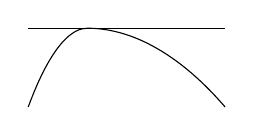
\begin{tikzpicture}
\drawaxis{-2}{4}{-0.5}{2};
\coordinate (c) at (1.25, 1.5);
\printcoordsonaxis{c}{c};

% рисуем кривую
\draw (0.5, 0.5) coordinate (a) parabola bend (c) (3, 0.5) coordinate (b);
\printcoordsonaxis{a}{a};
\printcoordsonaxis{b}{b}{f(a) = f(b)};

% рисуем касательную
\draw (c -| a) -- (c -| b);
\end{tikzpicture}
\end{wrapfigure}

\begin{proof}
Если $f(x) = f(a)$, то в~качестве точки~$c$ можно взять любую точку из~$(a; b)$.

Пусть $f(x)$ не является константой на~$[a; b]$, тогда по свойству~\ref{st:continuous_function_takes_inf_and_sup} непрерывной функции $\displaystyle \exists c \in (a; b) \colon \allowbreak f(c) \opbr= \inf_{x \in [a; b]} f(x) \lOr f(c) = \sup_{x \in [a; b]} f(x)$.
Для определённости предположим, что
\begin{equation*}
f(c) = \inf_{x \in [a; b]} f(x) \Leftrightarrow
\forall x \in [a; b] \ f(x) - f(c) > 0 \Rightarrow
\begin{cases}
\dfrac{f(x) - f(c)}{x - c} < 0, \ x < c \\
\dfrac{f(x) - f(c)}{x - c} > 0, \ x > c
\end{cases}
\end{equation*}

$f(x)$ дифференцируема в точке~$c$, тогда $\displaystyle \exists f'(c) = \lim_{x \to c} \frac{f(x) - f(c)}{x - c}$.
\begin{equation*}
\lim_{x \to c-0} \frac{f(x) - f(c)}{x - c} \leqslant 0 \lAnd
\lim_{x \to c+0} \frac{f(x) - f(c)}{x - c} \geqslant 0 \Rightarrow
f'(c) = 0
\end{equation*}

Доказательство в~случае $f(c) = \sup\limits_{x \in [a; b]} f(x)$ аналогично.
\end{proof}

\index{Теорема!Коши} \index{Теорема!о среднем}
\begin{theorem}[Коши о среднем значении]
\label{th:Cauchy's_mean_value}
Если функции $f(x)$ и $g(x)$ непрерывны на~$[a; b]$, дифференцируемы на~$(a; b)$, $g(a) \neq g(b)$, то
\begin{equation*}
\exists c \in (a; b) \colon \frac{f(b) - f(a)}{g(b) - g(a)} = \frac{f'(c)}{g'(c)}
\end{equation*}
\end{theorem}
\begin{proof}
Пусть
\begin{equation*}
F(x) = f(x) - \frac{f(b) - f(a)}{g(b) - g(a)}(g(x) - g(a))
\end{equation*}

$F(x)$ дифференцируема на~$(a; b)$, $F(a) = F(b) = f(a)$, тогда по теореме Ролля
\begin{equation*}
\exists c \in (a; b) \colon 0 = F'(c) = f'(c) - \frac{f(b) - f(a)}{g(b) - g(a)} g'(c) \Rightarrow
\frac{f(b) - f(a)}{g(b) - g(a)} = \frac{f'(c)}{g'(c)}
\end{equation*}
\end{proof}

\begin{theorem}[Лагранжа о среднем значении]
\label{th:mean_value}
Если функция~$f(x)$ непрерывна на~$[a; b]$, дифференцируема на~$(a; b)$, то
\begin{equation}
\label{eq:mean_value_formula}
\exists c \in (a; b) \colon f(b) - f(a) = f'(c)(b - a)
\end{equation}
\end{theorem}

\begin{center}
\begin{tikzpicture}
\drawaxis{-0.5}{6}{-0.5}{3};
\draw[name path=curve] (0.1, -0.5) to[out=75, in=-110] (0.4, 0.65) coordinate (a)
	to[out=70, in=-150] (1.3, 2) coordinate (c)
	to[out=30, in=135] (2.5, 1)
	to[out=-45, in=-120] (3.5, 1.5)
	to[out=60, in=-110] (4.2, 3)
	node[below right] {$y = f(x)$};
\printcoordsonaxis{a}{a};
\printcoordsonaxis{c}{c};
\draw (c) +(-150:2) -- +(30:3);

\path[name path=AB] (a) -- +(30:7);
\draw[name intersections={of=curve and AB, total=\t}]
	(a) -- (intersection-\t) coordinate (b);
\printcoordsonaxis{b}{b};
\end{tikzpicture}
\end{center}

\index{Формула!конечных приращений} Равенство~(\ref*{eq:mean_value_formula}) называется \textbf{формулой конечных приращений}.
\begin{proof}
Достаточно положить в теореме Коши $g(x) = x$.
\end{proof}

\subsection{Производные и дифференциалы высших порядков}
Производная произвольного порядка определяется рекуррентно:
\begin{equation*}
\forall n \in \mathbb N \ f^{(0)}(x) = f(x), \ f^{(1)}(x) = f'(x), f^{(2)}(x) = f''(x) \ f^{(n + 1)}(x) = (f^{(n)}(x))'
\end{equation*}

Также определяется дифференциал произвольного порядка:
\begin{equation*}
\forall n \in \mathbb N \ d^0 f(x) = f(x), \ df(x) = f'(x)dx, \ d^2 f(x) = f''(x) dx^2, \ d^n f(x) = f^{(n)}(x) dx^n
\end{equation*}

\subsection{Формула Тейлора}
\index{Формула!Тейлора}
\begin{theorem}[формула Тейлора]
\label{eq:Taylor_series}
Если функция~$f(x)$ в~некоторой окрестности~$U(a)$ имеет все производные порядка $n + 1$ и ниже, то
\begin{equation*}
\forall x \in U(a) \
f(x) = \sum_{k=0}^n \frac{f^{(k)} (x - a)^k}{k!} + R_n(x), \
R_n(x) = \frac{f^{(n + 1)}(a + \Theta(x - a))}{(n + 1)!}(x - a)^{n + 1}, \
\Theta \in (0; 1)
\end{equation*}
\end{theorem}

$R_n(x)$ называется \textbf{остаточным членом} в~форме Лагранжа и используется для оценки ошибки. Также его можно представить в~форме Пеано~--- $R_n(x) = o((x - a)^n)$~--- которая используется при вычислении пределов.

\index{Формула!Маклорена}
Подставив $a = 0$ в~формулу Тейлора, получим \textbf{формулу Маклорена}:
\begin{equation}
\label{eq:Maclaurin_series}
f(x) = \sum_{k=0}^n \frac{f^{(k)} x^k}{k!} + R_n(x), \
R_n(x) = \frac{f^{(n + 1)}(\Theta x)}{(n + 1)!}\,x^{n + 1}, \
\Theta \in (0; 1)
\end{equation}

\subsubsection{Разложения некоторых функций в ряд Маклорена}
\begin{itemize}
	\item $f(x) = e^x, \
	f^{(n)}(x) = e^x, \
	f^{(n)}(0) = 1$
	\begin{equation*}
	\forall n \in \mathbb N \ f(x) = 1 + x + \frac{x^2}{2!} + \ldots + \frac{x^n}{n!} + R_n(x), \
	R_n(x) = \frac{e^{\Theta x}}{(n + 1)!}\,x^{n + 1}
	\end{equation*}
	\begin{equation*}
	|R_n(x)| \leqslant e^{\max \{ 0, x \}} \cdot \frac{|x|^{n + 1}}{(n + 1)!} \Rightarrow
	\begin{cases}
	\displaystyle |R_n(x)| \leqslant \frac{|x|^{n + 1}}{(n + 1)!}, \ x < 0 \\
	\displaystyle |R_n(x)| \leqslant 3^x \cdot \frac{|x|^{n + 1}}{(n + 1)!}, \ x > 0
	\end{cases}
	\end{equation*}
	
	\item $f(x) = \sin x, \
	f^{(n)}(x) = \sin \left( x + \dfrac\pi{2} n \right), \
	f^{(n)}(0) = \sin \dfrac\pi{2} n =
	\begin{cases}
	0, \ n \mult 2 \\
	1, \ \exists k \in \mathbb Z \colon n = 4k + 1 \\
	-1, \ \exists k \in \mathbb Z \colon n = 4k + 3
	\end{cases}$
	\begin{equation*}
	\forall n \in \mathbb N \ f(x) = x - \frac{x^3}{3!} + \frac{x^5}{5!} - \ldots + \frac{(-1)^{n-1} \cdot x^{2n-1}}{(2n - 1)!} + R_n(x), \
	R_n(x) = \frac{\sin \left( \Theta x + \frac\pi2 (2n + 1) \right)}{(2n + 1)!}\,x^{2n+1}
	\end{equation*}
	\begin{equation*}
	|R_n(x)| \leqslant \frac{|x|^{2n+1}}{(2n + 1)!}
	\end{equation*}
	
	\item $f(x) = \cos x,
	f^{(n)}(x) = \cos \left( x + \dfrac\pi{2} n \right), \
	f^{(n)}(0) = \cos \dfrac\pi{2} n =
	\begin{cases}
	0, \ n \notmult 2 \\
	1, \ \exists k \in \mathbb Z \colon n = 4k \\
	-1, \ \exists k \in \mathbb Z \colon n = 4k + 2
	\end{cases}$
	\begin{equation*}
	\forall n \in \mathbb N \ f(x) = 1 - \frac{x^2}{2!} + \frac{x^4}{4!} - \ldots + \frac{(-1)^{n-1} x^{2n-2}}{(2n - 2)!} + R_n(x), \
	R_n(x) = \frac{\cos (\Theta x + \pi n)}{(2n)!}\,x^{2n}
	\end{equation*}
	\begin{equation*}
	|R_n(x)| \leqslant \frac{x^{2n}}{(2n)!}
	\end{equation*}
	
	\item $f(x) = \ln (1 + x), \
	f^{(n)}(x) = \dfrac{(-1)^{n-1} (n - 1)!}{(1 + x)^n}, \
	f^{(n)}(0) = (-1)^{n-1} (n - 1)!$
	\begin{equation*}
	\forall n \in \mathbb N \ f(x) = x - \frac{x^2}2 + \frac{x^3}3 - \ldots + \frac{(-1)^{n-1} x^n}n + R_n(x), x \in (-1; 1], \
	R_n(x) = \frac{(-1)^n x^{n+1}}{(n + 1)(1 + \Theta x)^{n+1}}
	\end{equation*}
	
	Для вычисления $\ln a$, $a \neq -1$, можно воспользоваться формулой
	\begin{equation*}
	\ln \frac{1 + x_0}{1 - x_0} = \ln (1 + x_0) - \ln (1 - x_0) =
	2 \left( x_0 + \frac{x_0^3}3 + \frac{x_0^5}5 + \ldots \right)
	\end{equation*}
	\begin{equation*}
	a = \frac{1 + x_0}{1 - x_0} \Leftrightarrow
	a - a x_0 = 1 + x_0 \Leftrightarrow
	x_0 = \frac{a - 1}{a + 1}
	\end{equation*}
	
	\item $f(x) = (1 + x)^\alpha, \
	f^{(n)}(x) = \alpha (\alpha - 1) (\alpha - 2) \cdot \ldots \cdot (\alpha - n + 1) (1 + x)^{\alpha - n}, \
	f^{(n)}(0) = \alpha (\alpha - 1) (\alpha - 2) \cdot \ldots \cdot (\alpha - n + 1)$
	\begin{equation*}
	\forall n \in \mathbb N \ f(x) = 1 + \alpha x + \frac{\alpha (\alpha - 1) x^2}{2!} + \ldots + \frac{\alpha (\alpha - 1) \cdot \ldots \cdot (\alpha - n + 1) x^n}{n!} + R_n(x), |x| < 1,
	\end{equation*}
	\begin{equation*}
	R_n(x) = \frac{\alpha (\alpha - 1) \cdot \ldots \cdot (\alpha - n) (1 + \Theta x)^{\alpha-n-1}}{(n + 1)!}\,x^{n+1}
	\end{equation*}
\end{itemize}

\subsection{Правило Лопиталя}
\begin{theorem}[правило Лопиталя]
Если
\begin{enumerate}
	\item $\displaystyle \lim_{x \to a} f(x) = \lim_{x \to a} g(x) = 0 \lOr
	\lim_{x \to a} f(x) = \lim_{x \to a} g(x) = \infty$
	\item $g'(x) \neq 0$
	\item $\displaystyle \exists \lim_{x \to a} \dfrac{f'(x)}{g'(x)}$	
\end{enumerate}
то $\displaystyle \lim_{x \to a} \dfrac{f(x)}{g(x)} = \lim_{x \to a} \dfrac{f'(x)}{g'(x)}$.
\end{theorem}

Если $f(x)$ и $g(x)$ непрерывны в~окрестности точки~$a$, то для случая $\lim\limits_{x \to a} f(x) = \lim\limits_{x \to a} g(x) = 0$ можно провести следующее доказательство:
\begin{equation*}
\lim_{x \to a} \frac{f(x)}{g(x)} =
\lim_{x \to a} \frac{f(x) - 0}{g(x) - 0} =
\lim_{x \to a} \frac{f(x) - f(a)}{g(x) - g(a)} \;
\left| \text{По \hyperref[th:Cauchy's_mean_value]{теореме Коши}} \right| =
\lim_{x \to a} \frac{f'(c)}{g'(c)} =
\end{equation*}
\begin{equation*}
\left| c \in (x; a) \lOr c \in (a; x) \right| =
\lim_{x \to a} \frac{f'(x)}{g'(x)}
\end{equation*}

Полное доказательство правила Лопиталя слишком сложно, поэтому здесь не приводится.